\documentclass{sig-alternate}
\usepackage[english]{babel}
%nastavenie cislovania
\pagenumbering{arabic}
\usepackage{url}
%grecka abeceda
\usepackage{textgreek}
\usepackage[utf8]{inputenc}
%knižnica na grafiku a opravenie float
\usepackage{graphicx,dblfloatfix}
\graphicspath{ {Images/} }
\usepackage{booktabs}
%knižnica pre popisy vnútry figure
\usepackage{caption}
\usepackage{float}
\setlength{\heavyrulewidth}{1.2pt}
\setlength{\lightrulewidth}{0.7pt}

\begin{document}
\setcounter{page}{135}
\title{Content Wizard: Concept-Based Recommender System for
Instructors of Programming Courses}

\numberofauthors{3}

\author{
\alignauthor
Hung Chau\\
       \affaddr{School of Information Sciences,}\\
       \affaddr{University of Pittsburgh}\\
       \affaddr{Pittsburgh, PA, USA}\\
       \email{hkc6@pitt.edu}
\alignauthor
Jordan Barria-Pineda\\
       \affaddr{School of Information Sciences,}\\
       \affaddr{University of Pittsburgh}\\
       \affaddr{Pittsburgh, PA, USA}\\
       \email{jab464@pitt.edu}
\alignauthor
Peter Brusilovsky\\
       \affaddr{School of Information Sciences,}\\
       \affaddr{University of Pittsburgh}\\
       \affaddr{Pittsburgh, PA, USA}\\
       \email{peterb@pitt.edu}
}
\maketitle

\begin{abstract}
Authoring an adaptive educational system is a complex process that
involves allocating a large range of educational content within a
fixed sequence of units. In this paper, we describe Content Wizard,
a concept-based recommender system for recommending learning
materials that meet the instructor’s pedagogical goals during the
creation of an online programming course. Here, the instructors
are asked to provide a set of code examples that jointly reflect the
learning goals that are associated with each course unit. The Wizard
is built on top of our course-authoring tool, and it helps to decrease
the time instructors spend on the task and to maintain the coherence
of the sequential structure of the course. It also provides instructors
with additional information to identify content that might be not
appropriate for the unit they are creating. We conducted an off-
line study with data collected from an introductory Java course
previously taught at the University of Pittsburgh in order to evaluate
both the practicality and effectiveness of the system. We found that
the proposed recommendation’s performance is relatively close to
the teach
\end{abstract}

%\category{TODO}{TODO}{TODO}
%\category{TODO}{TODO}{TODO}

%\terms{Design, Experimentation}

\keywords{Concept-based recommendation; course authoring; learning con-
tent recommendation}

\begin{figure*}[!t]
\centering
\begin{minipage}{.5\textwidth}
  \centering
  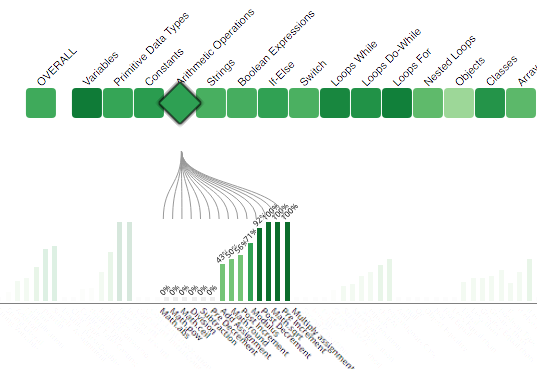
\includegraphics[width = \linewidth]{obr1.png}
  (a) Concept visualization of a specific course unit
\end{minipage}%
\begin{minipage}{.5\textwidth}
  \centering
  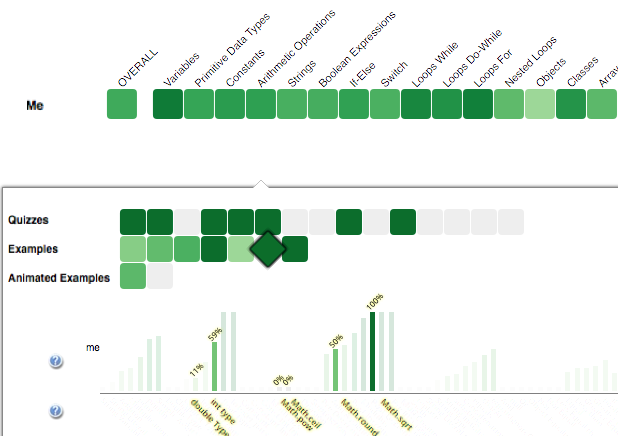
\includegraphics[width=\linewidth]{obr2.png}
  (b) Concept visualization of a specific learning activity
\end{minipage}
\captionof{figure}{Mastery Grids student interface}
\label{fig:fig1}
\end{figure*}
\section{Introduction}
Over the past twenty years, most of the intelligent tutoring Systems
(ITS) have focused their personalization efforts on helping students
to find an “optimal path” through available learning content to
achieve their learning goals. A range of personalization technolo-
gies, known as course sequencing, adaptive navigation support,
and content recommendation can now account for the learning
goals and the current state of student knowledge and recommend
the most appropriate content (e.g., a problem, an example, an educa-
tional video, etc.). However, in the context of real courses, there is
no complete freedom in selecting appropriate content for students.
An instructor usually plans a course as a sequence of topics to be learned. To stay in sync with the instructor and the class, students
are expected to work on course topics in the order determined by
the instructor’s plan. In this context, the personalized selection
of learning content should account for both a student’s prospects
(i.e., current knowledge levels) and the instructor’s prospects (the
preferred order of topics or learning goals).
Unfortunately, the current generation of adaptive learning sys-
tems rarely support an adaptation to a teacher’s preferences. In
most of these systems, a sequence of topics is predefined and learn-
ing content items are statically assigned to these topics. While
this approach works well for instructors who are happy to follow
the sequence of topics as defined by the ITS, any instructors who
prefer a different topic structure will find the system unacceptable,
since it does not support their approach to teaching the course.
These considerations are especially important when learning pro-
gramming. It is well-known that there are many ways to structure
a course that teaches the same programming language. Almost
every instructor and every textbook introduces a unique way of
course organization [11]. Throughout the last few years, we have
been developing an infrastructure that can support personalized
learning in this challenging context. Our infrastructure supports
authoring instructional content and creating diverse courses over
the same broad collection of learning materials, and is able to offer
personalization that considers both a student’s and an instructor’s
preferences. For course authors, our infrastructure offers tools for
both content and course authoring. We provide tools to create vari-
ous kinds of smart learning content, such as parameterized problems
[9] or annotated examples \cite{third}. We also provide a course-authoring
tool that allows instructors to define their preferred sequence of
topics and assign smart learning content to each topic. However,
our work with instructors revealed that the assistance provided by
the current course authoring tool is not sufficient. While defining
a sequence of topics is an easy task, selecting the most relevant
content for each topic is a real challenge. The instructors need
to carefully review a large number of content items in order to
select those items that fit their learning goals for the topic. This is
a time-consuming and error-prone process [12–14]. To offer better
support for instructors, we developed Content Wizard, a content
recommender system for instructors. The Wizard presented in this
paper uses a concept-based approach to recommend learning activ-
ities that are most appropriate to the instructors’ preferred model
of the course. We believe that this kind of recommender system is
vital to scale up teacher-adapted course authoring and to maintain
a coherent sequential structure of the personalized course.
We start our presentation of Content Wizard with a brief review
of related work. Details about Content Wizard and its current rec-
ommendation approach are presented in Section 3. In Section 4, we
describe our attempts to evaluate Content Wizard against a baseline.
Finally, Section 5 discusses the advantages and disadvantages of
our system, as well as plans for future work in this area.

\section{Context}
\begin{figure*}[b!]
\centering
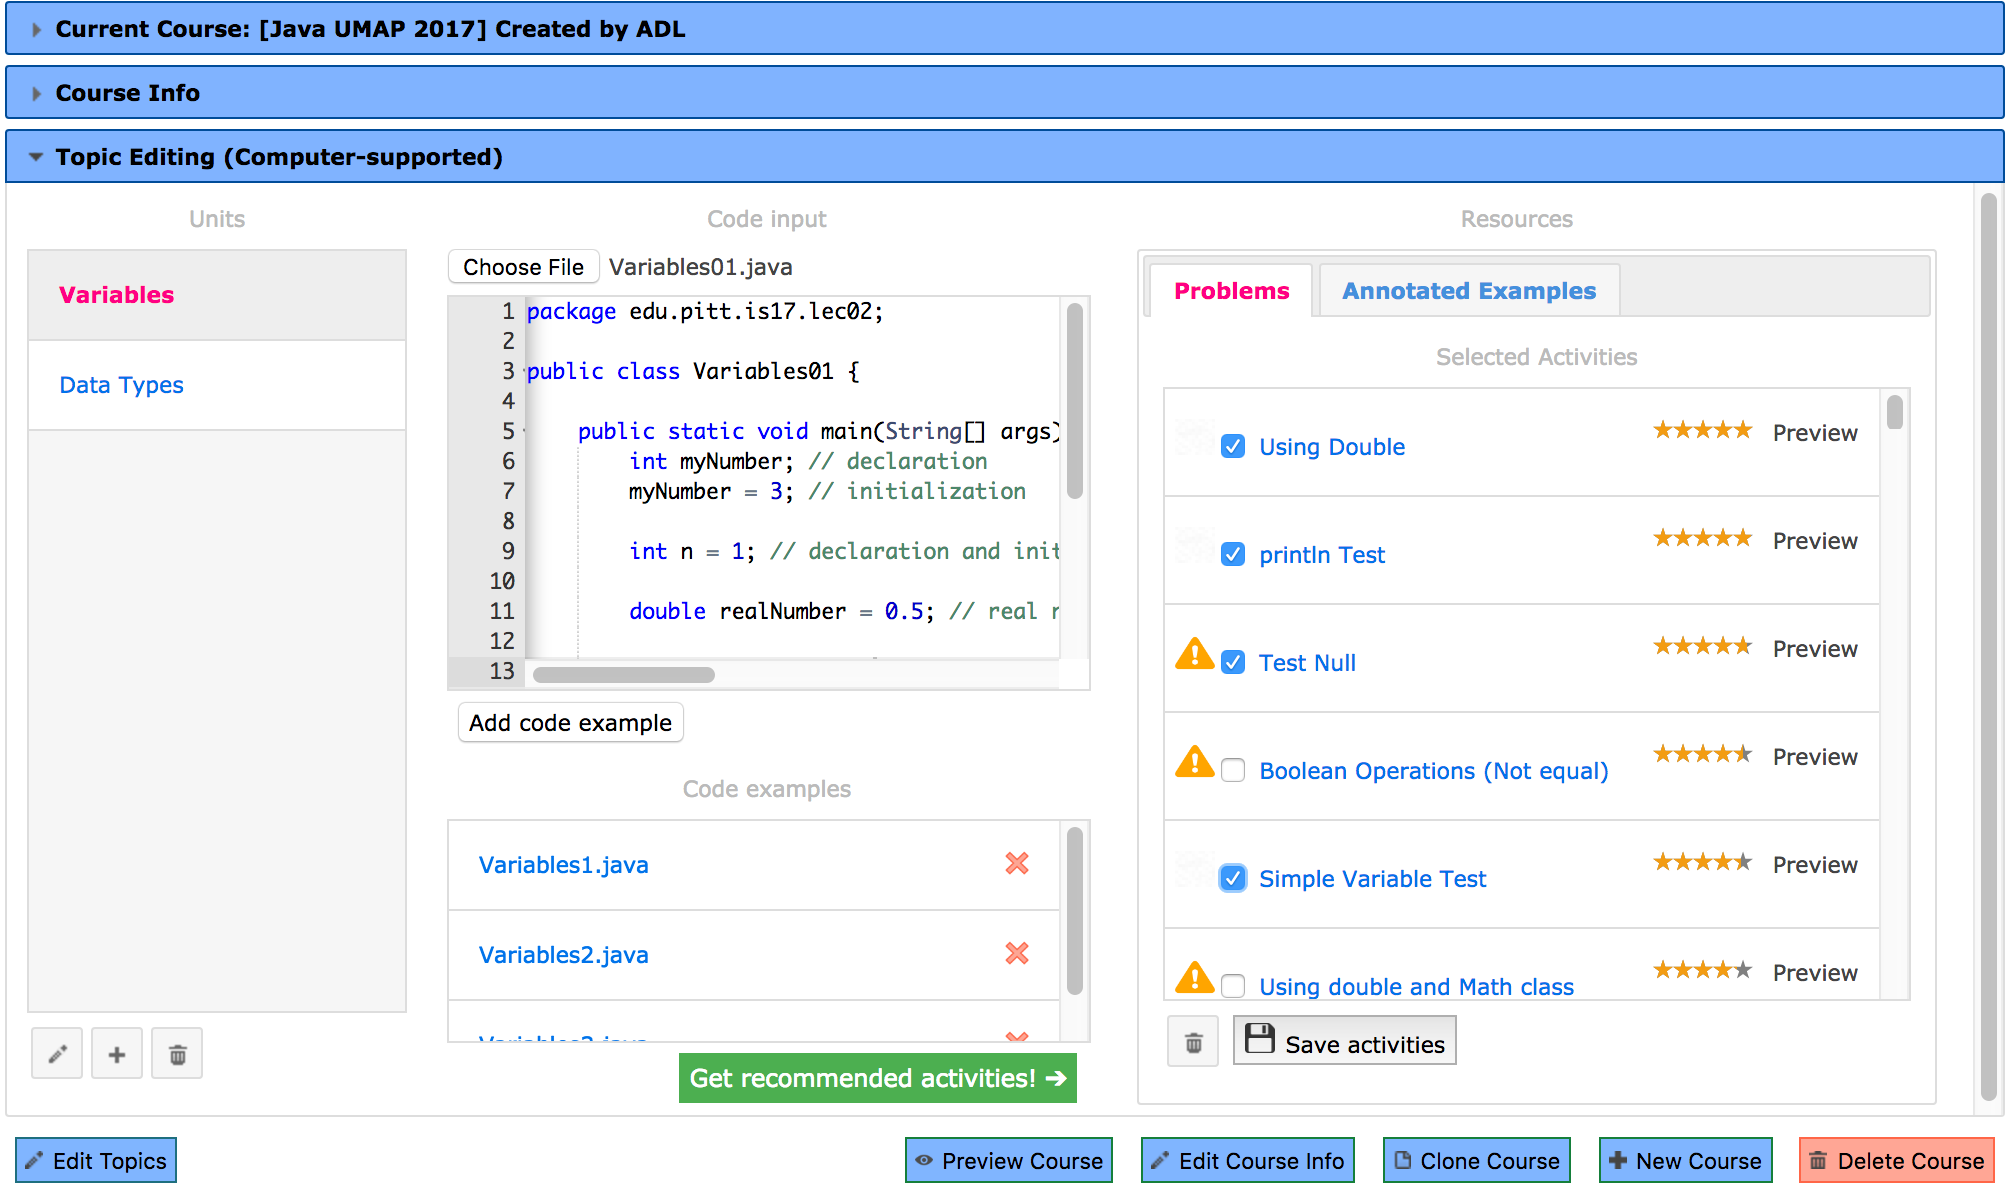
\includegraphics[width=170mm]{obr3.png}
\caption{Course Authoring Tool interface}
\label{fig:fig2}
\end{figure*}
Several systems have been developed to support the challenging
task of authoring in ITS context. Murray [12, 13] defines seven
categories of ITS authoring tools and generally classifies them into
two broad groups: pedagogy-oriented and performance-oriented
systems. Pedagogy-oriented systems focus on organizing instruc-
tional units and tutoring strategies. The instructional structure in
most of them usually is fairly simple; it includes, for example, a set
of instructional units that contains specific content (e.g. text, graph-
ics, examples and problems). These systems support instructors in
managing curriculum sequencing and planning, designing teach-
ing strategies and tactics, composing multiple knowledge types
(e.g., topics and concepts), and authoring adaptive hypermedia. On
the other hand, performance-oriented systems focus on provid-
ing a rich educational environment in which students can gain
problem-solving expertise, procedural skills, concepts, and facts
by practicing and receiving feedback and guidance from tutors.
Authoring tools in this group include simulation-based learning,
domain expert systems, and some special purpose systems.
ASPIRE, developed by Mitrovic et al.[10], is a performance-
oriented authoring system for a constraint-based ITS, which can be
used by instructors to author an ITS to supplement their courses.
ASPIRE is formed by an authoring server (ASPIRE-Author) and a tu-
toring server (ASPIRE-Tutor). ASPIRE-Author allows non-computer
scientists to develop new constraint-based tutors with main support
for generating the domain model and producing a fully functional
system. Another performance-oriented authoring tool is cognitive
tutor authoring tools (CTAT) \cite{first}, which allow authors to develop
two types of tutors: cognitive tutors and example tracing tutors.
CTAT was developed to support problem-based task domains. The CTAT authoring process requires authors to give a definition of
a task domain (such as the fraction addition problem) along with
appropriate problems. On the other hand, Situate Pedagogical Au-
thoring (SitPed) \cite{fourth} is a pedagogy-oriented authoring system that
supports instructors in creating simple, hierarchical task models;
authoring assessment knowledge; and creating tutor feedback and
guidance. It also provides predefined scenario files that are pre-
sented to learners in specific tasks.
Just a few previous research efforts have focused on assisting
teachers in tasks related to the design of adaptive online courses.
Cristea and Aroyo \cite{fifth} defined guidelines for developing adaptive
authoring tools for adaptive educational hypermedia, emphasiz-
ing that learning content has to be defined at the concept level,
in order to allow the system to structure the course and recom-
mend the most appropriate activities to include. Brusilovsky et al.
\cite{second} addressed this challenge by allowing teachers to design C pro-
gramming courses through the specification of a sequential set of
knowledge concepts linked by prerequisite-outcome relationships
that define the structure of the course. However, they did not im-
plement a complete system for supporting the whole process, from
defining the course concepts’ sequence to delivering the course
with the complete set of learning activities included.
Our current work in this area is focused on supporting instruc-
tors to develop adaptive educational systems and courses that are
able to recommend the most appropriate learning activities. Most
recently, we developed Mastery Grids \cite{sixth}, an intelligent course-
level user interface that supports personalized access to a collection
of learning activities related to the programming domain. Mastery
Grids incorporates open student modeling and social comparison to
increase student performance and engagement during the learning
process. In Mastery Grids, every course is visualized as a sequence
of instructor-defined course topics (i.e., learning goals) represented
as squares (see Figure \ref{fig:fig1}). By clicking on a specific course topic,
students can access a range of interactive learning activities that
can allow them to practice knowledge associated with the topic (see Figure
\ref{fig:fig1}). The system guides the student to the most appropriate
learning content using open student modeling (the intensity of the cell color reflects the the progress of student knowledge of the topic;
see Figure \ref{fig:fig1}), social comparison [6], and direct recommendation
[8].

While our main focus was on student-level personalization, our
experience revealed that the quality of recommendation and navi-
gation support in this context depends on the quality of the course
structure; namely, the sequence of topics and the content allocation.
Our experience with developing several courses for Mastery Grids
(Java, Python, and SQL) also highlighted challenges that instruc-
tors have to face when authoring an online programming course.
This work involves answering several questions, including: How
can the course be divided into the most appropriate sequence of
units? Which learning activities should be offered for each topic to
support students in achieving the anticipated learning goals of this
topic? How can we ensure that the content offered in the earlier
topics enables students to master all the types of knowledge that
are necessary to work with the current topic? To support our own
work on course authoring, we developed an authoring tool that
provided some level of support in defining the course structure. Yet,
as our work with other instructions demonstrated, the basic level
of support was not sufficient. The Content Wizard presented in this
paper augments the course authoring tool with a concept-based
recommender system that assists instructors in designing courses
according to their own expectations and pedagogical strategies.
Similar to most of the authoring tools described in this section,
our proposed system aims to decrease the effort required to build
an ITS (e.g. time and cost), and facilitating the task of maintaining a
coherent sequential structure of an adaptive educational system. In
particular, we enhance two beneficial characteristics of authoring
tools: reusing learning content to reduce the burden of creating
a content space [13, 14] and supporting knowledge management and visualization that helps authors understand and comprehend a
large amount of complex knowledge [13].

\section{Content Wizard}

Content Wizard is a recommender system that support instructors
in structuring online content for their courses by recommending
the most suitable learning content to include for each unit of the
envisioned course. The key idea of the system is to deduce the con-
cept structure of the envisioned courses by analyzing the content of
program examples that an instructor plans to present for each unit.
Content Wizard works at the top level of our course authoring tool
(see Figure \ref{fig:fig2}).
\subsection{Course Generation}
Each of the stages of this workflow are explained below. For a
better understanding, sequential steps in the diagram of Figure \ref{fig:fig3}
are colored from light gray (step 1) to dark gray (step 6).
\begin{figure*}[t!]
\centering
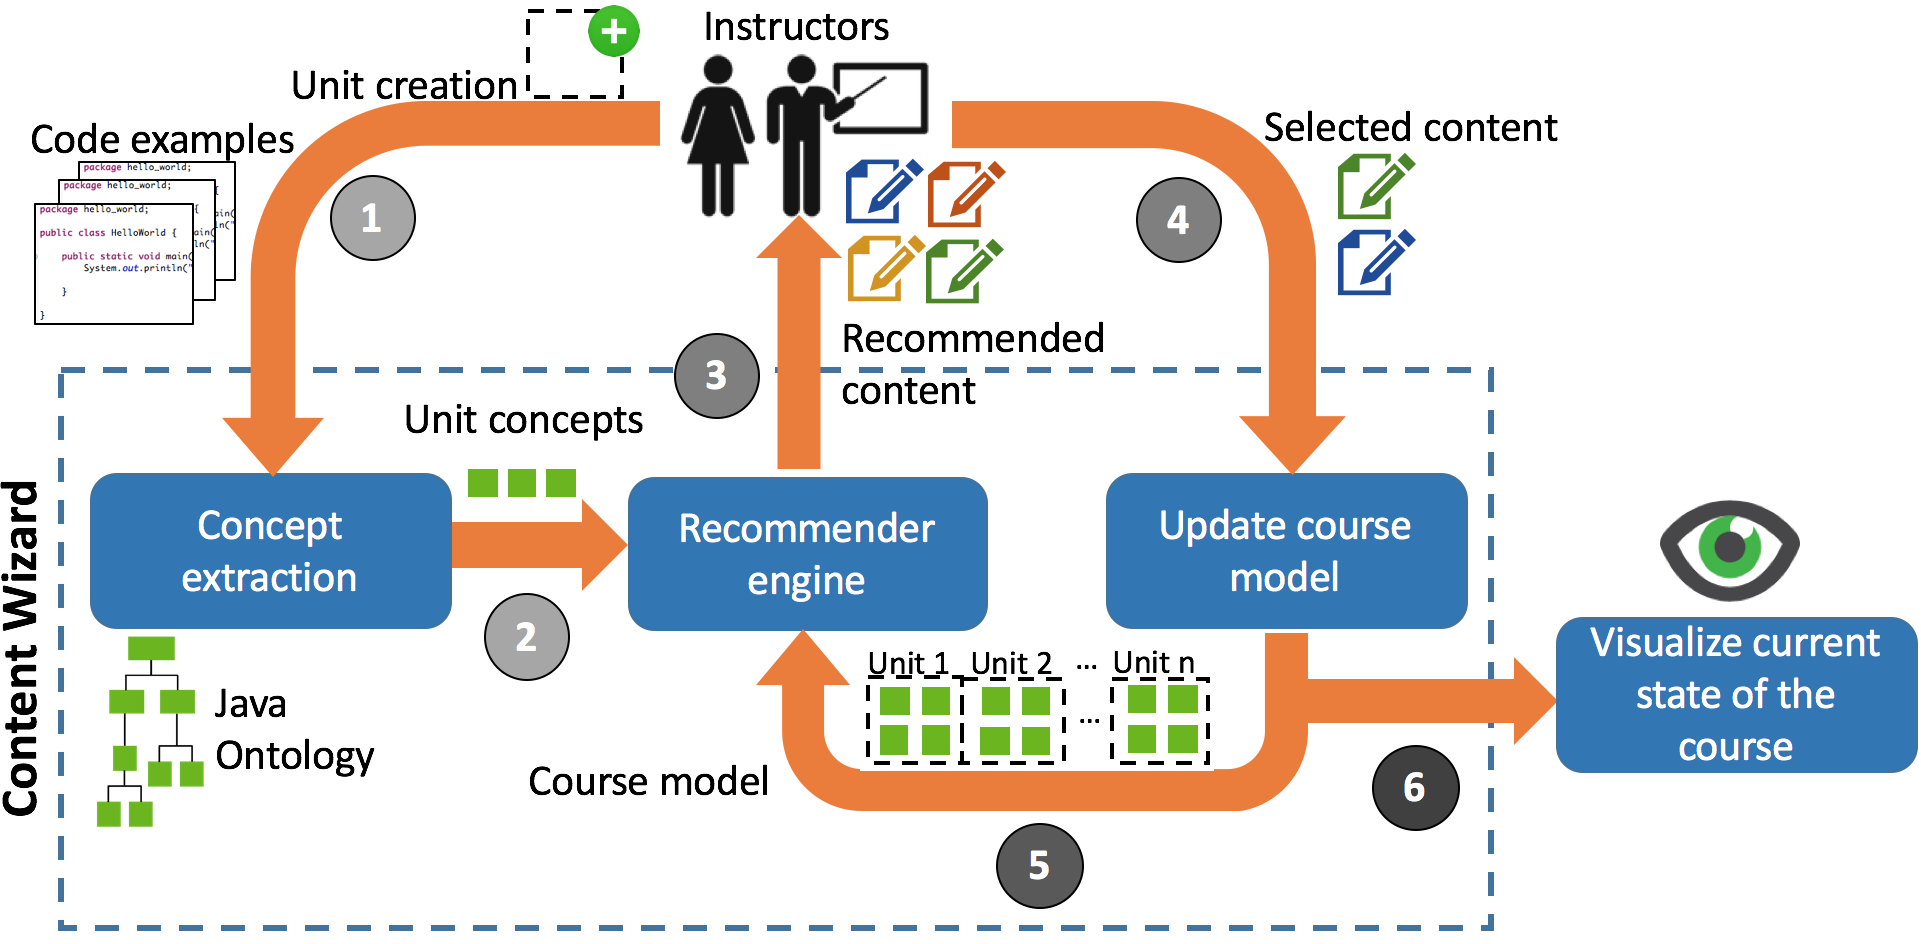
\includegraphics[width=160mm]{obr4.png}
\caption{Content Wizard workflow diagram}
\label{fig:fig3}
\end{figure*}
\begin{enumerate}
  \item The instructor creates a new course unit with a set of learning
goals in mind. To communicate the intended goals of the unit,
she uploads a set of code examples that she uses during the
lecture to introduce the concepts of the unit.
  \item Content Wizard automatically extracts the Java programming
concepts that are associated with each code example. This
extraction is performed by using a Java parser [7], which works
based on an ontology of fine-grained programming concepts
(e.g. a For Loop)\footnote{http://www.sis.pitt.edu/ ∼ paws/ont/java.owl} . For each unit, it forms the set of covered
concepts that merges concepts from all unit examples.
\item The authoring tool accesses external services for providing dif-
ferent types of learning content. Our providers are Quiz Jet (parameterized semantics Java problems) and W ebEx (interac-
tive annotated Java code examples). Content Wizard queries
this content to pick up the most relevant items for each sec-
tion. Considering the set of concepts covered in the current
unit and the set of knowledge concepts that have been covered
in previous created units, the system ranks all the available
learning activities in order to highlight the material that best
fits the instructor’s needs. The recommendation process will
be described in detail in Section 3.2.
\item The instructor examines the retrieved ranked list and selects
the learning activities that she thinks are more appropriate to
add to the new course unit.
\item The current course model is updated in order to include the
new knowledge concepts related to this unit that have appeared
for the first time in the course. The course model is defined as
the set of concepts covered throughout the course, which are
ordered according to the first unit in which they appeared as
part of its learning material.
\item During any step of the process, instructors are able to have a
preview of the current state of the course by visualizing it as
how it would look when linked to the Mastery Grids system
(see Figure \ref{fig:fig1}). In this way, we provide a visualization of how
the units of the created course are linked with the concepts
that are associated with the learning material that has been
included in each of them (see Figure \ref{fig:fig1}). Users can access this
functionality by clicking the button ”Preview course” in the
Figure \ref{fig:fig2}.
\end{enumerate}
\begin{figure*}[!t]
\centering
\begin{minipage}{\textwidth}
  \centering
  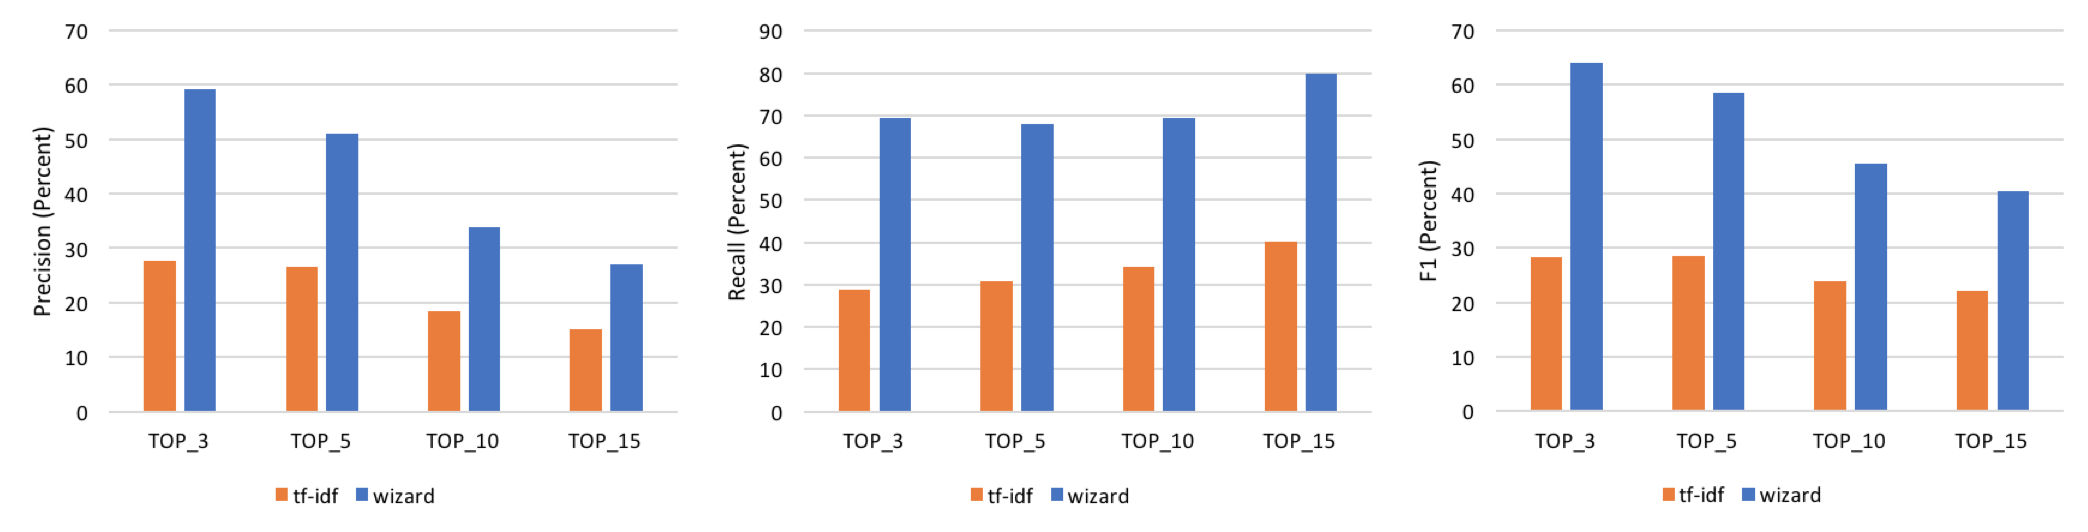
\includegraphics[width = \linewidth]{obr5.png}
  (a) Annotated Example
\end{minipage}%

\begin{minipage}{\textwidth}
  \centering
  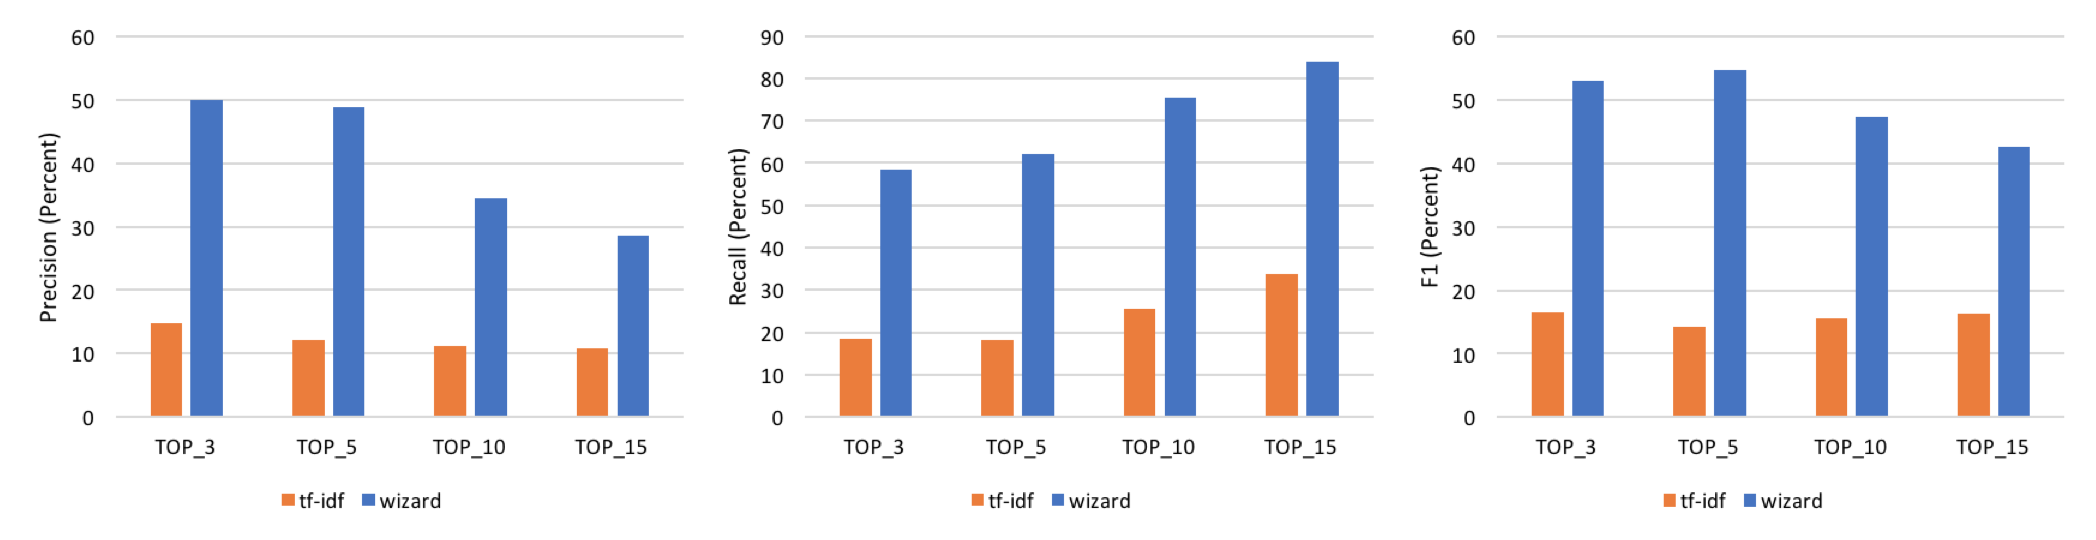
\includegraphics[width=\linewidth]{obr6.png}
  (b) Quiz
\end{minipage}
\captionof{figure}{Performance comparison of the Content Wizard and the baseline.}
\label{fig:fig4}
\end{figure*}
\subsection{Recommendation algorithm}

The recommendations for each iteration of the course creation
process are calculated by considering two main factors: the current
structure of the course (course model) and the type of learning
content they want to teach on each course unit. These two factors
are described in terms of knowledge programming concepts.
Content Wizard adaptively provides two valuable sources of
information that can help instructors find the most appropriate
contents for each unit: a ranking list and warning flags. At every
step of course generation, the concepts extracted from the code
examples provided for the ongoing created unit are classified in
three categories that help to determine the suitableness of adding
the remaining learning content to the current unit, according to
the sequence of concepts covered in the course at that stage. These
three categories are:
\begin{itemize}
\item Last concepts (P): Concepts that were already covered in previous
units. These concepts are supposed to be known before starting
the current unit. We assign a low positive impact to this set of
concepts because it is not necessarily harmful to the students to
practice them again, even when the instructor wants to focus on
teaching new concepts.
\item Current concepts (C): Concepts that are covered in the current
unit (according to the examples), but that have not been covered
in any previous units. We consider these concepts as targets of
the current unit according to the instructor’s vision of the course.
We assign them a high positive impact on students’ learning.
\item Future concepts (F): Concepts that that are not covered by the
current unit and any previous unit. We assume that the instructor
prefers to cover these concepts in future units (or not to cover
them at all). Most likely, these concepts are not yet appropriate
for students to learn in that part of the course. Thus, we assign
them a negative impact.
\end{itemize}
We calculate the ranking score of each learning activity a i by
linearly combining the contribution of the concepts it covers ac-
cording to the category to which they belong. In this context, C i
is a subset of the current concept set C, P i is a subset of the past
concept set P, and F i is a subset of the future concepts set F ; these
concepts appear in a i . Equation (1) shows how we compute each
content ranking score:
\begin{equation}
    {score_a}_i =  \alpha |C_i|+ \beta|P_i|+ \gamma|F_i|  \quad    
\alpha = 1, \beta = 0.2, \gamma = -1.5
\end{equation}
For setting \textalpha , \textbeta , and \textgamma values in Equation (1), we assigned them
initial values based on our assumptions about the importance of
each concept category. Then, we collected a set of code examples
from a Java programming book and ran the algorithm using this
formula, while adjusting the parameter values in order to get the
best recommendation results (by taking the book’s contents as
ground truth). It is important to note that there are no optimal
values for the parameters in Equation (1), since each instructor
perceives the importance of each type of concepts in a different
way.
According to the ranking scores, we sort the available learning
content in descending order. Content that has a high score is a
better candidate for satisfying instructor needs.
Further, we think it is important for instructors to identify the
learning content that, even though it fits well with the learning
goals they defined for the current unit, presents one or more ad-
ditional knowledge concepts that could potentially interfere with
the achievement of the desired outcomes. Thus, we identify these
activities by applying Equation (2) to each activity.
\begin{equation}
    {warning_a}_i =   \begin{Bmatrix}1,&if|F_i|>0\\0&otherwise\end{Bmatrix}
\end{equation}
If the activity a i has a warninд value of 1 (see Equation 2), we
highlight it graphically using a yellow warning icon (see the third,
fourth, and sixth rows in Figure \ref{fig:fig2}), in order to tell them that the
activity may contain additional concepts that are not found within the code examples and the previous units. The instructor can then
evaluate if the additional concepts should be included within the
unit.
\section{Evaluation}

To evaluate our proposed system, we use data from two Java classes
taught in the School of Information Sciences at the University
of Pittsburgh in Fall 2016 (referred as IS17F16). The instructors
followed a lecture-based format and created a course structure
for IS17F16 that includes 18 units. The Content Wizard has not
been used to create the course. The course was released to the
students through Mastery Grids system. To run the study, we, firstly,
collected the code examples provided by the teachers in order to use
them as inputs for running the recommendation process. After that,
we created a new course with the same structure. For each unit, we
provided the corresponding code examples to get the recommended
contents from the pool of more than 300 contents, and then compare
them to the ones the instructors picked themselves for the IS17F16
course.\\
\quad Considering code examples as a query formed by concepts and
each content item as a document in the Java programming domain,
we apply TF-IDF method as a baseline and run the same process to
get a set of recommended items. In this process, we also treat each
content item as a list of concepts extracted by the same parser and
then calculate the TF-IDF weighting for each concept within that
content. To measure the performance of both our method and the baseline, we use the three classical metrics: precision, recall, and
F1 score (at top 3, top 5, top 10, and top 15).
As shown in Figure \ref{fig:fig4}, the Content Wizard consistently outper-
forms the TF-IDF method with all the metrics, as well as with the
different kinds of content (i.e., annotated examples and problems).
Moreover, the Wizard performs similarly for both types of content;
it suggests that our method could apply to other kinds of educa-
tional items (such as animated examples). The Wizard also achieves
good recall performance (69.44% to 79.78% for annotated examples,
and 58.48% to 84.05% for problems), much higher than those of
the baseline (28.7% to 40.1% for annotated examples, and 18.57% to
33.89% for problems). The precision is less impressive (27.04% to
59.26% for annotated examples, and 28.5% to 50% for problems), but
still much better than the baseline (15.18% to 27.78% for annotated
examples, and 10.74% to 14.82% for problems). However, the lower
precision is typical for an off-line cross-validation study. The reason
for the low precision levels is that the goal of the instructors when
creating the course was to select some relevant content for each
unit, but not all relevant content. Since our content repository
includes a much larger volume of content than is necessary for a
single course, only a subset of all relevant items was selected for the
course. To obtain a better understanding of the overall performance
of the Content Wizard, we plan further experiments, which are
discussed in the next section.
\section{DISCUSSION AND FUTURE WORK}
In this work, we presented a concept-based recommender system for recommending learning content that is relevant to teachers’
preferences in authoring programming courses. It was designed
to reduce time and effort spent by instructors in selecting content
for each course unit. Each content item is represented as a list
of fine-grained concepts to make a recommendation. However, it
can be argued that some concepts are more important than others
in the same learning item (the document in general). Exploring
the importance of each concept and adding its weighting to the
Equation (1) may potentially help the Content Wizard archive a
better ranking.
Moreover, by observing the automatically deduced course struc-
ture that was produced in our study, we noticed that although in
most of the cases the concepts from the code examples cover all the
concepts from the content selected by the instructors, some con-
cepts such as PostIncrementExpression (+=) do appear in the selected
content, but are not found in any provided code examples (though
these do contain the concept PostDecrementExpression (-=)). While
a group of related concepts is usually introduced in the same unit,
only some of these concepts are usually illustrated in the exam-
ples. The lack of knowledge about the relationship between similar
concepts clearly affects system performance. Therefore, we plan to
add the relationships between concepts in the future version of the
recommender system.
As mentioned in the previous section, since we ran an off-line
study that uses the real course designed to tutor the students to
evaluate the Content Wizard, our results might not reveal the actual
performance of the model. We plan to run an online experiment;
first, we will collect the textbook and materials that instructors use
to teach their classes as the inputs; then we will send the whole recommended courses to them; and finally, we will ask them to
evaluate the content that the Wizard recommended. Through this
process, it will help us to have a thorough understanding of the
performance of our system. Additionally, we aimed at building a
recommender system that provided different support to teachers.
For instance, besides the ranking list, we also display the visualiza-
tion of the authored course and mark some content with warning
signs. A warning sign tells the instructor that a content contains
concepts that may not be appropriate for the current unit, because
the concepts are not included either in the code examples or in pre-
vious units. The usefulness of these features cannot be evaluated in
the off-line study. Improving the overall accuracy of the recommen-
dations is not the only goal of our work; in the future, we are also
planning to add features that contribute to the transparency of the
recommendation process and perform a more extensive evaluation
of the new tool.

\begin{thebibliography}{14}
\bibitem{first} 
Vincent Aleven, Bruce M. McLaren, Jonathan Sewall, and Kenneth R. Koedinger.
2006. The Cognitive Tutor Authoring Tools (CTAT): Preliminary Evaluation of
Efficiency Gains. In \textit{Proceedings of the 8th International Conference on Intelligent
Tutoring Systems}  (ITS’06). Springer-Verlag, Berlin, Heidelberg, 61–70.
\bibitem{second} 
Peter Brusilovsky, Sergey Sosnovsky, Michael Yudelson, and Girish Chavan. 2005.
Interactive Authoring Support for Adaptive Educational Systems. In Proceedings
of the 2005 Conference on AIED: \textit{Supporting Learning Through Intelligent and
Socially Informed Technology. } IOS Press, Amsterdam, The Netherlands, 96–103.
\bibitem{third} 
Peter Brusilovsky and Michael V. Yudelson. 2008. From WebEx to NavEx: Inter-
active Access to Annotated Program Examples. \textit{ Proc. IEEE} 96, 6 (2008), 990–999.
\bibitem{fourth}
H. Chad Lane, Mark G. Core, Matthew J. Hays, Daniel Auerbach, and Milton
Rosenberg. 2015. Situated Pedagogical Authoring: Authoring Intelligent Tutors
from a Student’s Perspective. \textit{In Artificial Intelligence in Education,}  Vol. 9112.
Springer International Publishing, Madrid, Spain, 195–204.
\bibitem{fifth}
Alexandra I. Cristea and Lora Aroyo. 2002. Adaptive Authoring of Adaptive
Educational Hypermedia. In \textit{Proceedings of the Second International Conference on
Adaptive Hypermedia and Adaptive Web-Based Systems (AH ’02)} . Springer-Verlag,
London, UK, UK, 122–132.
\bibitem{sixth}
Julio Guerra, Roya Hosseini, Sibel Somyurek, and Peter Brusilovsky. 2016. An
Intelligent Interface for Learning Content: Combining an Open Learner Model
and Social Comparison to Support Self-Regulated Learning and Engagement. In \textit{Proceedings of the 21st International Conference on Intelligent User Interfaces (IUI
’16)}
. ACM, New York, NY, USA, 152–163.

\end{thebibliography}
\balancecolumns

\end{document}
